\documentclass{article}

\usepackage{tikz}
\usetikzlibrary{patterns}

%-------------------------------------------------------
%: xmin xmax ymin ymax
\tikzset { xmin/.store in=\xmin, xmin/.default=-3, xmin=-3,
           xmax/.store in=\xmax, xmax/.default=3, xmax=3,
           ymin/.store in=\ymin, ymin/.default=-3, ymin=-3,
           ymax/.store in=\ymax, ymax/.default=3, ymax=3}

%: domaine
\tikzset {domaine/.style 2 args={domain=#1:#2}}

%: Commande \grille : trace la grille entre (xmin,ymin) et (xmax,ymax)
\newcommand {\grille} {\draw[help lines] (\xmin,\ymin) grid (\xmax,\ymax);}

%: Commande \axes
\newcommand{\axes}
{\draw[->] (\xmin,0) -- (\xmax,0); \draw[->] (0,\ymin) -- (0,\ymax);}

%: Commande \fenetre : limite de l'affichage (xmin,ymin) et (xmax,ymax)
\newcommand {\fenetre} {\clip (\xmin,\ymin) rectangle (\xmax,\ymax);}

%-------------------------------------------------------
\begin{document}

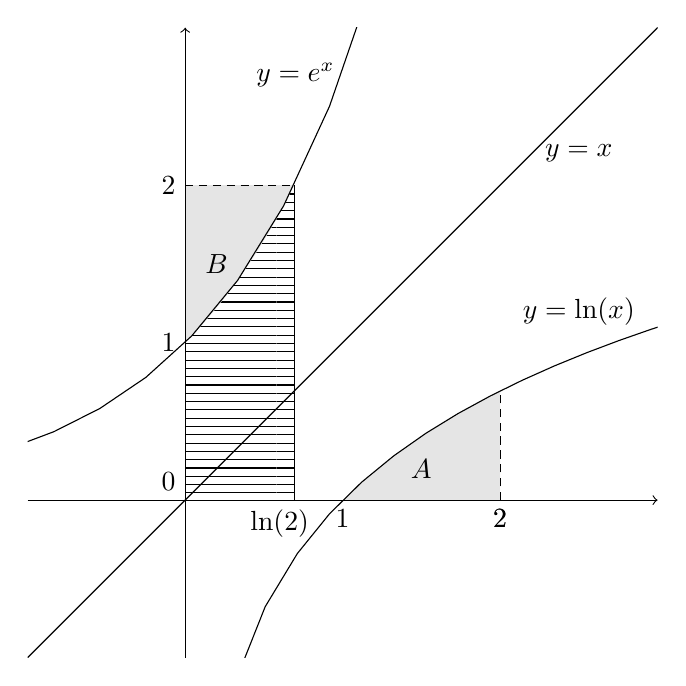
\begin{tikzpicture}[scale=2,xmin=-1,xmax=3,ymin=-1,ymax=3]
  \fenetre
  \fill [fill=gray!20]
    plot [domaine={1}{2}] (\x,{ln(\x)}) -- (2,0) node [below] {$2$} -- cycle;
  \fill [fill=gray!20] 
    plot [domaine={0}{ln(2)}] (\x,{exp(\x)}) -- (0,2) -- cycle;
  \fill [pattern= horizontal lines]
    (0,0) -- plot [domaine={0}{ln(2)}] (\x,{exp(\x)}) -- ({ln(2)},0) -- cycle;
  \axes
  \draw plot [domaine={0.1}{5}] (\x,{ln(\x)});
  \draw plot [domaine={-2}{5}] (\x,{exp(\x)});
  \draw plot [domaine={-2}{5}] (\x,\x);
  \draw  ({ln(2)},0) -- ({ln(2)},2);
  \draw (0.6,0) node[below] {$\ln(2)$};
  \draw [densely dashed] (2,0) -- (2,{ln(2)}) (0,2) -- ({ln(2)},2);
  \draw (0,0) node[above left]{$0$};
  \draw (0,1) node[left]{$1$};
  \draw (0,2) node[left] {$2$};
  \draw (1,0) node[below] {$1$};
  \draw (2,0) node[below] {$2$};
  \draw (2.5,2.2) node {$y=x$};
  \draw (2.5,1.2) node {$y=\ln(x)$};
  \draw (0.7,2.7) node {$y=e^x$};
  \draw (1.5,0.2) node{$A$} (0.2,1.5) node {$B$};
\end{tikzpicture}

\end{document}
